%# -*- coding: utf-8-unix -*-
%%==================================================
%% thesis.tex
%%==================================================

% 双面打印
\documentclass[master, fontset=adobe, openright, twoside, zihao=-4]{sjtuthesis}
% \documentclass[bachelor, fontset=adobe, openany, oneside, submit]{sjtuthesis}
% \documentclass[master, fontset=adobe, review]{sjtuthesis}
% \documentclass[%
%   bachelor|master|doctor,	% 必选项
%   fontset=adobe|windows,  	% 只测试了adobe
%   oneside|twoside,		% 单面打印,双面打印(奇偶页交换页边距,默认)
%   openany|openright, 		% 可以在奇数或者偶数页开新章|只在奇数页开新章(默认)
%   zihao=-4|5,, 		% 正文字号:小四、五号(默认)
%   review,	 		% 盲审论文,隐去作者姓名、学号、导师姓名、致谢、发表论文和参与的项目
%   submit			% 定稿提交的论文,插入签名扫描版的原创性声明、授权声明 
% ]

% 逐个导入参考文献数据库
\addbibresource{bib/thesis.bib}
% \addbibresource{bib/chap2.bib}

\begin{document}

%% 无编号内容:中英文论文封面、授权页
%# -*- coding: utf-8-unix -*-
\title{SSD缓存系统的设计与实现}
\author{傅雨东}
\advisor{李小勇}
% \coadvisor{某某教授}
\defenddate{2018年1月15日}
\school{上海交通大学}
\institute{网络空间安全学院}
\studentnumber{115036910016}
\major{计算机科学与技术}

\englishtitle{The Design and Implement of Solid State Disk Cache System}
\englishauthor{\textsc{Fu Yudong}}
\englishadvisor{\textsc{Li Xiaoyong}}
% \englishcoadvisor{Prof. \textsc{Uom Uom}}
\englishschool{Shanghai Jiao Tong University}
\englishinstitute{\textsc{School of Cyber Security} \\
  \textsc{Shanghai Jiao Tong University} \\
  \textsc{Shanghai, P.R.China}}
\englishmajor{Computer Science and Technolgy}
\englishdate{Jan. 15th, 2018}


\maketitle

\makeenglishtitle

\makeatletter
\ifsjtu@submit\relax
	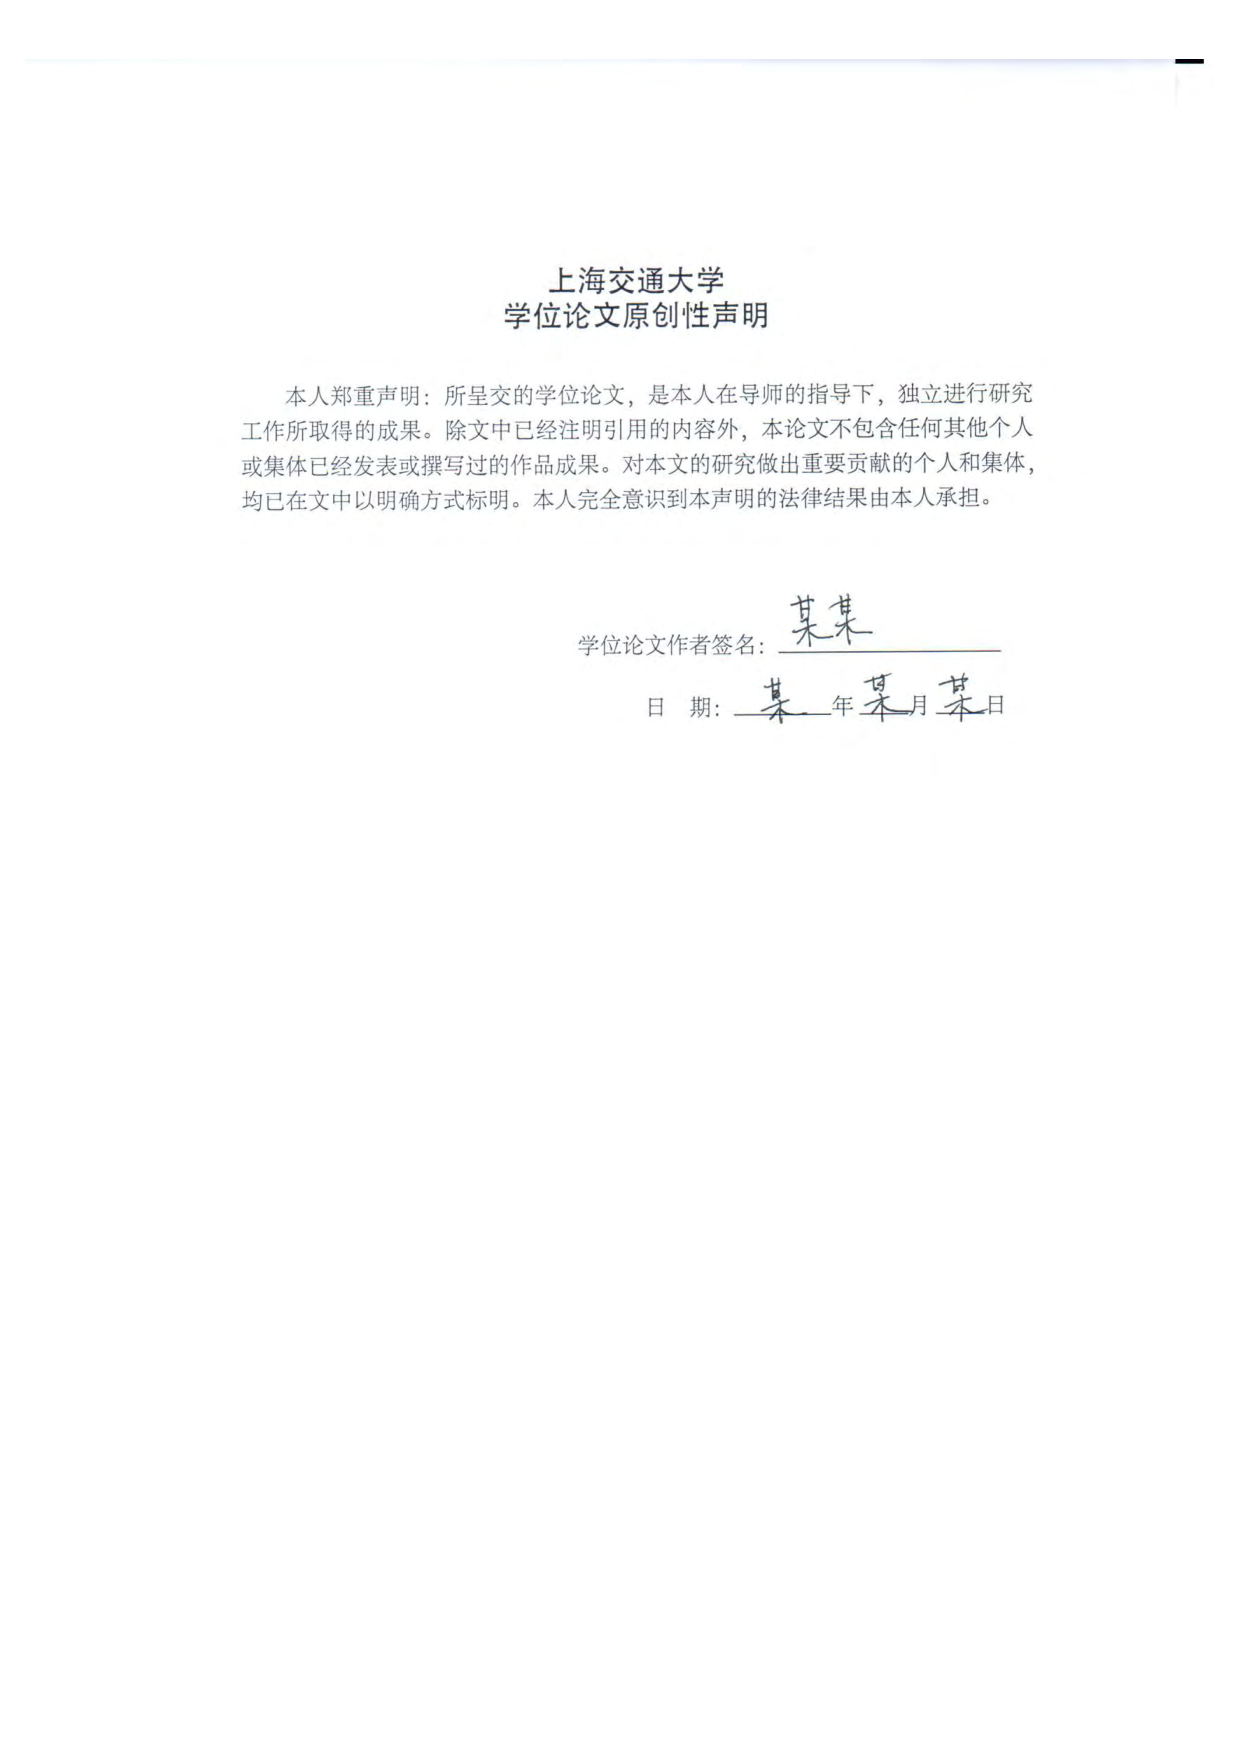
\includepdf{pdf/original.pdf}
	\cleardoublepage
	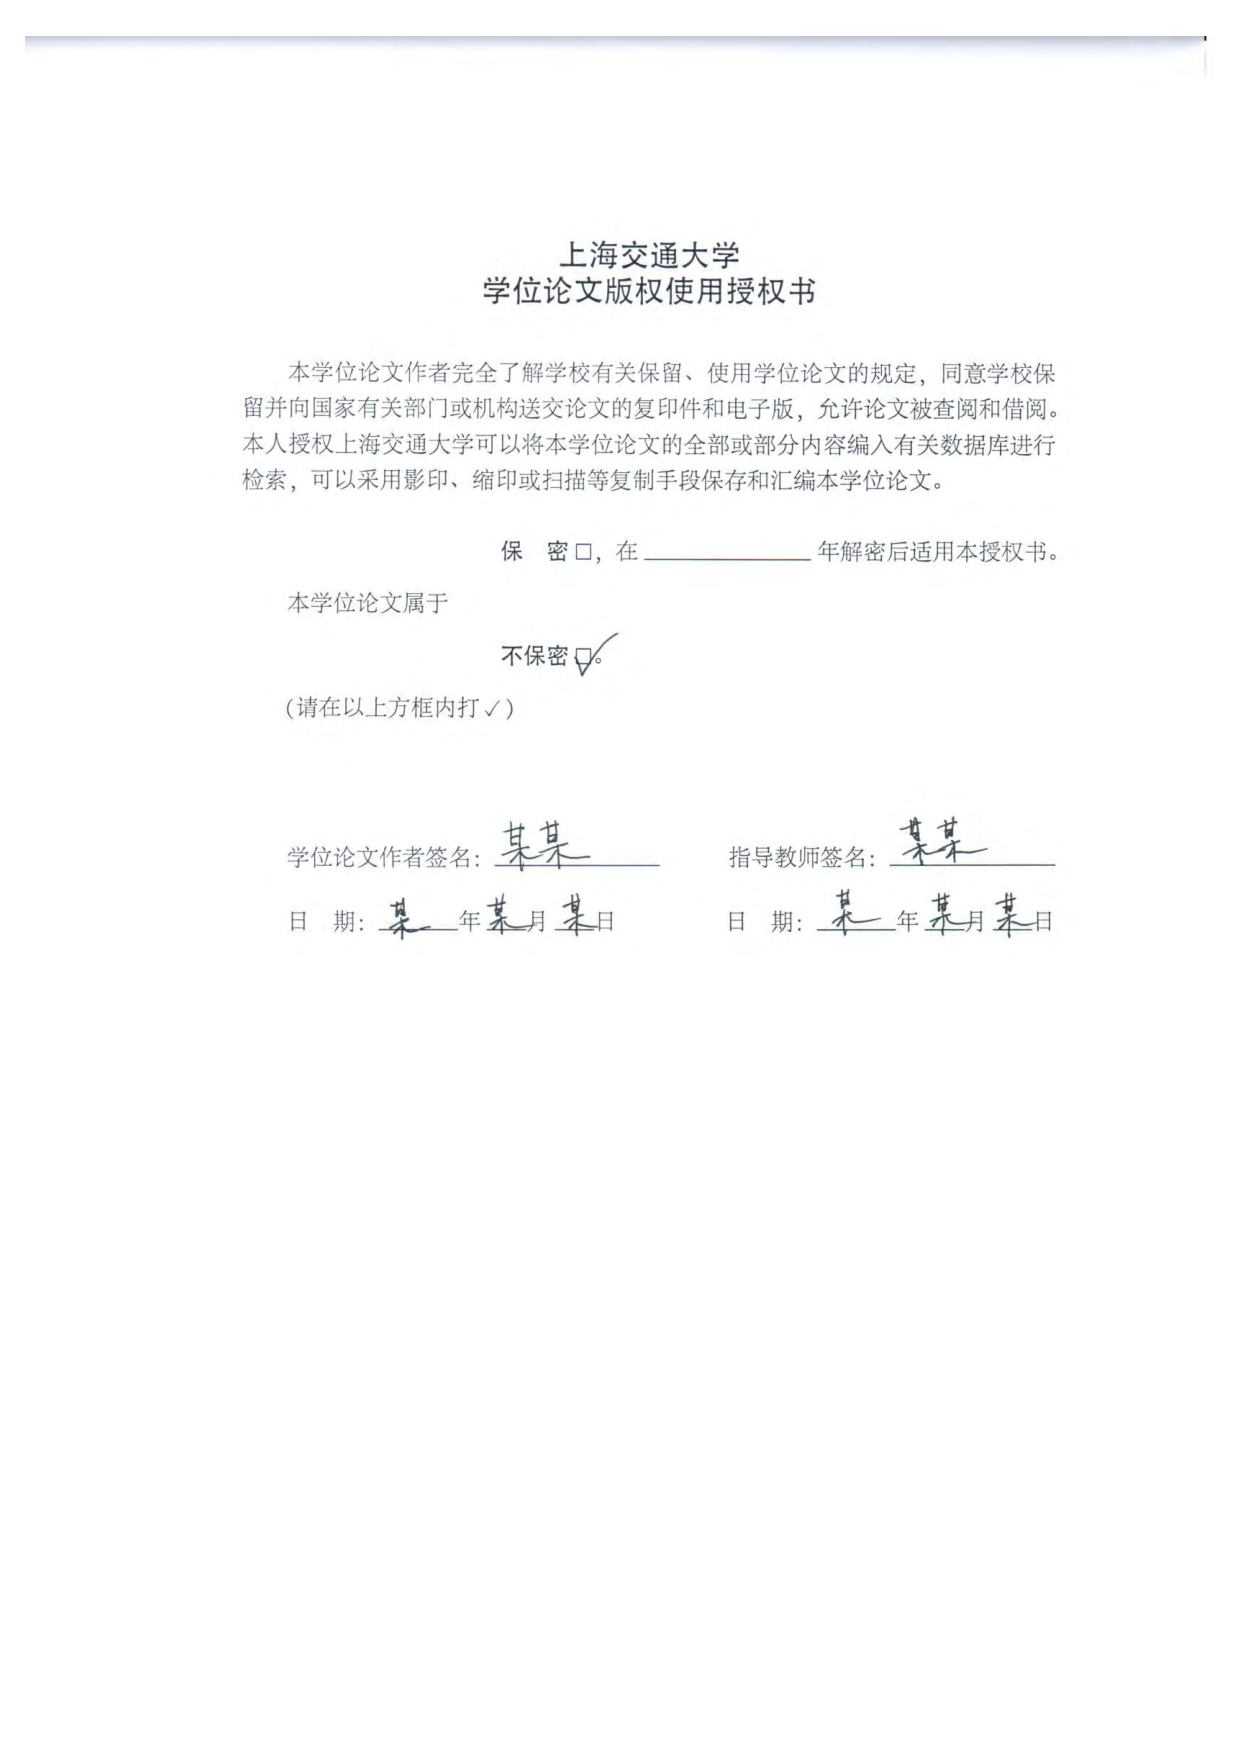
\includepdf{pdf/authorization.pdf}
	\cleardoublepage
\else
\ifsjtu@review\relax
% exclude the original claim and authorization
\else
	\makeDeclareOriginal
	\makeDeclareAuthorization
\fi
\fi
\makeatother


\frontmatter 	% 使用罗马数字对前言编号

%% 摘要
\pagestyle{main}
%# -*- coding: utf-8-unix -*-
%%==================================================
%% abstract.tex for SJTU Master Thesis
%%==================================================

\begin{abstract}

随着云计算与大数据的快速发展,对作为其基石的存储系统的要求越来越高,存储系统需要具备大容量、低成本、高性能。而目前主流的任何一种存储设备如固态盘、磁盘由于各种限制不能单独构建出同时满足上述要求的存储系统。混合存储系统充分利用不同存储设备特性的互补构建高效的存储系统,既能支持大容量,又能在保证系统低成本下仍能具有高性能,成为目前的研究热点。

本文首先介绍了混合存储系统的基本概念和发展历史,然后研究了混合存储系统在设计中的关键技术,之后研究了三个开源混合存储系统,在此基础上设计并实现了一个基于SSD和HDD的SSD缓存系统qscache。本文的主要工作如下:

\begin{enumerate}
    \item 对当前主流的存储设备介绍,并对性能、成本、容量进行了分析对比。
    \item 对混合存储系统的发展历史进行了研究并分析总结了混合存储系统在设计中的关键技术。
    \item 对三个开源混合存储系统进行了研究,分析对比了它们的性能和特性。
    \item 设计并实现了qscache系统。
    \item 对qscache系统的性能以及多缓存设备对多后台设备功能和对I/O带宽按权限分配的功能进行了测试。
\end{enumerate}

测试结果显示qscache系统的整体性能与flashcache接近,并且成功实现对I/O带宽按权限分配的功能,系统通过Linux内核模块实现,但需要对Linux内核进行修改。本论文的研究成果对于其它的混合存储系统设计与实现以及需要对Linux中Device Mapper进行功能扩展与修改的研究具有较好的借鉴价值。

\keywords{\large 混合存储 \quad 固态盘 \quad 磁盘 \quad 按权限配额}
\end{abstract}

\begin{englishabstract}

With the rapid development of cloud computing and big data, the storage system, which is the cornerstone, needs to provide high storage capacity and high performance at low cost. While at present any one of the storage devices, such as solid state disk and hard disk drive, can not meet the above requirements alone due to various limitations. Hybrid storage system takes full advantage of the characteristics of different storage device to support large-capacity, but also ensures high performance at low cost. Therefore, hybrid storage system is becoming the current research focus. 

This paper introduces the basic concepts and development history of hybrid storage system first, then studies the key technologies in the design of hybrid storage system, and then studies three open source hybrid storage systems, based on which, a hybrid storage system named qscache is designed and implentmented. The main work of this paper is as follows:

\begin{enumerate}
    \item The current wide-used storage devices are introduced, and their performance, cost, capacity were analyzed and compared.
    \item The history of the development of hybrid storage systems was studied and the key technologies in the design of hybrid storage systems were summarized.
    \item Three open source hybrid storage systems were studied, and their performance and characteristics were analyzed and compared.
    \item The design and implementation of hybrid storage system qscache.
    \item The performance of the qscache system, as well as the ability of support of multiple cache devices to multiple backend devices and the support of assigning I / O bandwidth based on weight, was tested.
\end{enumerate}

The test results shows that the performance of the qscache system is close to flashcache, and assigning I / O bandwidth based on weight is implemented. The qscache system is implemented as a kernel module in Linux, but the modification of Linux kernel is a must. This research provides a reference for the design and implementation of other hybrid storage systems and the modification of the Device Mapper in Linux kernel.

\englishkeywords{\large hybrid storage, solid state disk, hard disk drive, weight-based quota}
\end{englishabstract}



%% 目录、插图目录、表格目录
\tableofcontents
\listoffigures
\addcontentsline{toc}{chapter}{\listfigurename} %将插图目录加入全文目录
\listoftables
\addcontentsline{toc}{chapter}{\listtablename}  %将表格目录加入全文目录
\listofalgorithms
\addcontentsline{toc}{chapter}{算法索引}        %将算法目录加入全文目录

%%# -*- coding: utf-8-unix -*-
\chapter{主要符号对照表}
\label{chap:symb}

\begin{longtable}{rl}
$\epsilon$     & 介电常数 \\
 $\mu$ 		& 磁导率 \\
 $\epsilon$     & 介电常数 \\
 $\mu$ 		& 磁导率 \\
 $\epsilon$     & 介电常数 \\
 $\mu$ 		& 磁导率 \\
 $\epsilon$ 	& 介电常数 \\
 $\mu$ 		& 磁导率 \\
 $\epsilon$     & 介电常数 \\
 $\mu$ 		& 磁导率 \\
 $\epsilon$     & 介电常数 \\
 $\mu$ 		& 磁导率 \\
 $\epsilon$     & 介电常数 \\
 $\mu$ 		& 磁导率 \\
 $\epsilon$ 	& 介电常数 \\
 $\mu$ 		& 磁导率 \\
 $\epsilon$     & 介电常数 \\
 $\mu$ 		& 磁导率 \\
 $\epsilon$     & 介电常数 \\
 $\mu$ 		& 磁导率 \\
 $\epsilon$     & 介电常数 \\
 $\mu$ 		& 磁导率 \\
 $\epsilon$ 	& 介电常数 \\
 $\mu$ 		& 磁导率 \\
 $\epsilon$     & 介电常数 \\
 $\mu$ 		& 磁导率 \\
 $\epsilon$     & 介电常数 \\
 $\mu$ 		& 磁导率 \\
 $\epsilon$     & 介电常数 \\
 $\mu$ 		& 磁导率 \\
 $\epsilon$ 	& 介电常数 \\
 $\mu$ 		& 磁导率 \\
 $\epsilon$     & 介电常数 \\
 $\mu$ 		& 磁导率 \\
 $\epsilon$     & 介电常数 \\
 $\mu$ 		& 磁导率 \\
 $\epsilon$     & 介电常数 \\
 $\mu$ 		& 磁导率 \\
 $\epsilon$ 	& 介电常数 \\
 $\mu$ 		& 磁导率 \\
 $\epsilon$     & 介电常数 \\
 $\mu$ 		& 磁导率 \\
 $\epsilon$     & 介电常数 \\
 $\mu$ 		& 磁导率 \\
 $\epsilon$     & 介电常数 \\
 $\mu$ 		& 磁导率 \\
 $\epsilon$ 	& 介电常数 \\
 $\mu$ 		& 磁导率 \\
 $\epsilon$     & 介电常数 \\
 $\mu$ 		& 磁导率 \\
 $\epsilon$     & 介电常数 \\
 $\mu$ 		& 磁导率 \\
 $\epsilon$     & 介电常数 \\
 $\mu$ 		& 磁导率 \\
\end{longtable}
 % 主要符号、缩略词对照表

\mainmatter	% 使用阿拉伯数字对正文编号

%% 正文内容
\pagestyle{main}
%# -*- coding: utf-8-unix -*-
%%==================================================
%% chapter01.tex for SJTU Master Thesis
%%==================================================

%\bibliographystyle{sjtu2}%[此处用于每章都生产参考文献]
\chapter{绪论}
\label{chap:intro}

\section{研究背景与意义}

\subsection{研究背景}
\label{sec:backgrounds}

大规模分布式存储系统是是云计算与大数据的基石,是近年来的研究热点。随着近年来云计算与大数据的兴起,现有的存储设备正面临着诸多挑战。首先,随着数据量的爆发式增长,对存储系统的容量提出了更高的要求,如何在提供大容量存储的前提下尽可能降低成本是一大挑战\cite{gray2003next}。其次,由于云计算中的多台虚拟机可能会依赖于同一存储系统,这就导致该存储系统的负载整体会表现为随机化与碎片化,这对存储系统的随机读写性能有很高要求。最后,至今计算性能可谓日益提高,相比最初已有了巨大的提升,但存储设备的读写性能提高仍然有限,这就导致计算性能与存储性能之间的差距越来越巨大\cite{morris2003evolution},如何能提供与计算性能相匹配的存储设备的读写性能也是另一大挑战。

根本上来看,存储系统所基于的存储设备极大地决定了存储系统的性能。目前,磁盘(HDD:Hard Disk Drive)仍然是存储系统中最广泛使用的存储设备,虽然随着各种硬件技术的发展,磁盘的容量依然依照摩尔定律\cite{schirle1996history}在过去的30多年中增长了近十万倍,但是由于其磁头是机械移动这一根本性的限制,磁盘的访问延迟在过去的30年中仅提高了约2倍,而如果通过提高转速来进一步提高磁盘的访问性能,过高的转速会引发能耗与散热等诸多问题,因此磁盘的容量与访问性能之间的鸿沟十分巨大。

近年来,SSD(Solid State Disk,也被称为固态盘)这一新型存储设备的飞速发展为提升存储系统的性能提供了新的研究方向。与磁盘不同,SSD是电子器件,不像磁盘需要磁头的机械移动,因此SSD的随机读写性能要远胜于磁盘,另外由于没有磁头的机械移动,SSD相比磁盘的能耗更低,另外也更具抗震性。然而SSD仍有诸多问题。首先,虽然SSD相比磁盘在随机读写上性能要优秀得多,然而在顺序读写上性能相比磁盘并没有明显的优势。其次,SSD的成本相比磁盘仍要高出许多。最后,SSD的读写性能并不对称,这是由于SSD的写操作造成的,SSD对数据进行更新时需要首先将新数据写入空闲页面,然后将原页面标记为invalid,之后等待将原页面擦除后再将新数据写入原页面,最终导致SSD的写操作耗时约为读操作的6倍,并且由于SSD的擦除操作具有约五万次的次数限制,超出次数后的页面将无法使用,因此会带来耐久性问题。虽然SSD有上述几个问题,但SSD的优缺点与磁盘的优缺点可以很好地互补,因此将SSD与磁盘结合使用为设计大容量、高性能、低成本的存储系统提供了新的可能。

\subsection{研究意义}

目前在学术界与产业界,混合存储系统的研究越发受到重视,各方面的研究都有在开展。但是对于混合存储系统的研究仍然有些问题,主要体现在以下两个方面:

一方面,总的来看,学术界目前对于混合存储系统的研究尚处于起步阶段,很多工作的重点并不在于混合存储系统的设计与实现,而主要在关注SSD的物理结构与特性,关于基于SSD与磁盘的混合存储系统的文献\cite{guerra2011cost, kim2011hybridstore, 杨濮源2012一种时间敏感的, 陈震37基于磁盘和固态硬盘的混合存储系统研究综述}能公开搜索到的很少。另外在少数提出的基于SSD与磁盘的混合存储系统的文献中,真正进行了测试验证的文献更少,更多的是仅仅提供一种思路,无法验证其正确性。产业界中由一些国际一流的存储设备厂商推出的存储产品中已经有开始使用基于SSD与磁盘的混合存储设计,但这些存储设备的内部实现由于厂商并未公开相应资料因而无从知晓,性能的提升仅能依赖于一些简单的测试而并不能得知各项具体的性能提升数值。

另一方面,由于之前提到的SSD的擦除次数限制,这就导致在混合存储系统的写操作面临两难的境地:如果对于数据的写操作都在SSD中进行,那么势必会影响SSD的寿命,而如果将数据的写操作放到磁盘进行,那么势必会影响混合存储系统整体的写性能。因此目前混合存储系统的设计中仍有问题尚待解决。

因此,把握住SSD这一新型存储器件带来的机遇,开展基于SSD与磁盘的混合存储系统的研究,一方面是对于存储系统基础理论的创新,另一方面也对提升我国存储领域的核心竞争力具有重大意义。更进一步,也是为当下以及未来,我国云计算与大数据的发展打下坚实的存储基础。

\section{研究内容与目标}

本文将通过学习存储相关理论,并结合现有的混合存储系统实例分析,研究混合存储系统中的关键技术,在此基础上设计实现以SSD作为磁盘缓存的SSD缓存系统,对其进行测试、完善和优化,并与其它软件进行比较测试。

本文主要将包括以下三大目标:
\begin{enumerate}
    \item SSD、磁盘的随机读写性能、顺序读写性能、容量、成本的对比分析。
    \item 现有混合存储系统的随机读写性能、顺序读写性能、可靠性、额外开销的对比分析。
    \item 混合存储系统设计中的关键技术研究。
    \item 设计并实现一个基于SSD与磁盘的混合存储系统
\end{enumerate}

\section{论文结构}

论文正文分为七个章节,各章的内容安排如下: 

第一章:绪论。给出了论文的研究背景及意义,阐述了论文课题的研究内容和目标,最后说明了论文的组织结构。 

第二章:混合存储系统介绍。介绍了混合存储系统的概念,对当前主流的存储设备的特性进行了介绍,并对混合存储系统的发展历程进行了介绍。 

第三章:混合存储系统设计中的关键技术研究。本章节从系统架构、数据映射策略、冷热数据识别策略、数据写回/迁移策略、最优化存储设备组合这五个方面展开分析了混合存储系统设计中的关键技术。 

第四章:开源混合存储系统介绍。本章节对于目前主流的三个开源的混合存储框架进行了对比分析。

第五章:系统设计。首先介绍了qscache系统的设计目标与设计思想,然后介绍了qscache系统的系统架构、数据映射策略、冷热数据识别策略、数据写回/迁移策略、最优化存储设备组合等设计。 

第六章:系统实现。首先对于系统实现过程中需要掌握的预备知识进行介绍,然后对系统中一些关键问题的具体实现方法进行阐述。 

第七章:系统测试。首先介绍了系统测试的目标与测试方法,然后对于qscache系统的性能与功能进行测试,最后进行了小结。 

第八章:总结与展望。对论文所做的工作进行了总结,并且展望了将来可能的改进工作与改进方向。


%# -*- coding: utf-8-unix -*-
%%==================================================
%% conclusion.tex for SJTUThesis
%% Encoding: UTF-8
%%==================================================

%\begin{summary}

\chapter{总结与展望}
\label{chap:summary}

\section{全文总结}

本文针对基于混合存储系统,首先介绍了混合存储系统的基本概念和发展历史,然后研究了混合存储系统在设计中的关键技术,研究了三个开源的混合存储系统flashcache、dm-cache和bcache,分析对比了它们的特性和性能,然后设计并实现了一个基于SSD和HDD的混合存储系统qscache,最后对系统的性能进行了测评,并对系统对多缓存设备对多后台设备以及对I/O带宽按权限分配的功能进行了测试验证。具体工作如下:

\begin{enumerate}
    \item 介绍了混合存储系统产生的原因以及基本概念,并结合当前主流的存储设备介绍了混合存储系统的发展历史。
    \item 介绍了混合存储系统在设计中的关键技术,包括系统架构、数据映射策略、冷热数据识别策略、数据写回/迁移策略、最优化存储设备组合这五大方面。
    \item 介绍了三个开源混合存储系统flashcache、dm-cache和bcache并对它们的性能和特性进行了分析对比。
    \item 详细介绍了qscache系统的设计。首先介绍了系统的设计动机和设计目标然后对系统架构、数据映射策略、冷热数据识别策略、数据写回/迁移策略、最优化存储设备组合这五个关键问题展开介绍,另外对按权限分配I/O带宽的功能的设计进行了介绍。
    \item 详细介绍了qscache系统的实现。首先对系统实现过程中需要用到的预备知识进行了简单的介绍,然后针对系统的编程实现进行展开详细的介绍。
    \item 对qscache系统进行了测试。首先使用对比的方法,对基于HDD的系统、flashcache和qscache分别测试了它们在顺序读写性能和随机读写性能上的差异,然后验证了qscache对多缓存设备对多后台设备以及对I/O带宽按权限分配的功能的实现。
\end{enumerate}

\section{研究展望}

本文虽然已经取得了一些研究成果,但仍然存在可以进一步改进的内容:

\begin{enumerate}
    \item 目前qscache系统支持按权限分配不同的I/O带宽,但是仅仅只是限制了不同权限的进程能被分配到的IOPS不同,而对混合存储系统而言最重要的资源是缓存,目前qscache系统尚不支持针对不同权限的进程能按权限比例限制进程占有的缓存空间。在接下来的研究中考虑针对不同的权限分别维护一个LRU链表,每次有进程启动则针对该进程的权限慢慢将分配给它的缓存块划入对应的LRU链表管理,不同LRU链表按照不同权限设置不同的最大长度,这样不同权限的进程能得到的最大缓存块数量就实现了按权限分配。
    \item 目前qscache系统虽然支持多缓存设备对多后台设备,但是仍然是静态配置,需要在系统初始化时进行配置,而不能在系统运行过程中动态地增加缓存设备或后台设备。这个问题比较复杂,动态地扩容不仅影响设备的管理也会影响数据映射、冷热数据识别等多个方面,需要在之后的研究中进一步改进。
    \item 目前qscache系统虽然性能基本能达到flashcache的水平,但性能并没有达到理论极限,因此在后续研究中需要针对数据映射策略、冷热数据识别策略、数据写回/迁移策略这几个策略进行改进,进一步提升系统性能。
    \item 目前qscache仍只是单台机器的混合存储系统,而不支持分布式存储下的混合存储,后续研究中可以针对分布式存储环境下的混合存储技术展开进一步研究。
\end{enumerate}

%\end{summary}


\appendix	% 使用英文字母对附录编号,重新定义附录中的公式、图图表编号样式
\renewcommand\theequation{\Alph{chapter}--\arabic{equation}}	
\renewcommand\thefigure{\Alph{chapter}--\arabic{figure}}
\renewcommand\thetable{\Alph{chapter}--\arabic{table}}
\renewcommand\thealgorithm{\Alph{chapter}--\arabic{algorithm}}

%% 附录内容,本科学位论文可以用翻译的文献替代。
%%# -*- coding: utf-8-unix -*-
\chapter{搭建模板编译环境}

\section{安装TeX发行版}

\subsection{Mac OS X}

Mac用户可以从MacTeX主页\footnote{\url{https://tug.org/mactex/}}下载MacTeX 2015。
也可以通过brew包管理器\footnote{\url{http://caskroom.io}}安装MacTeX 2015。

\begin{lstlisting}[basicstyle=\small\ttfamily, numbers=none]
brew cask install mactex
\end{lstlisting}

\subsection{Linux}

建议Linux用户使用TeXLive主页\footnote{\url{https://www.tug.org/texlive/}}的脚本来安装TeXLive 2015。
以下命令将把TeXLive发行版安装到当前用户的家目录下。
若计划安装一个供系统上所有用户使用的TeXLive,请使用root账户操作。

\begin{lstlisting}[basicstyle=\small\ttfamily, numbers=none]
wget http://mirror.ctan.org/systems/texlive/tlnet/install-tl-unx.tar.gz
tar xzvpf install-tl-unx.tar.gz
cd install-tl-20150411/
./install-tl
\end{lstlisting}

\section{安装中文字体}

\subsection{Mac OS X、Deepin}

Mac和Deepin用户双击字体文件即可安装字体。

\subsection{RedHat/CentOS用户}

RedHat/CentOS用户请先将字体文件复制到字体目录下,调用fc-cache刷新缓存后即可在TeXLive中使用新字体。

\begin{lstlisting}[basicstyle=\small\ttfamily, numbers=none]
mkdir ~/.fonts
cp *.ttf ~/.fonts				# 当前用户可用新字体
cp *.ttf /usr/share/fonts/local/	# 所有用户可以使用新字体
fc-cache -f
\end{lstlisting}


%%# -*- coding: utf-8-unix -*-
%% app2.tex for SJTU Master Thesis
%% based on CASthesis
%% modified by wei.jianwen@gmail.com
%% version: 0.3a
%% Encoding: UTF-8
%% last update: Dec 5th, 2010
%%==================================================

\chapter{Maxwell Equations}

选择二维情况,有如下的偏振矢量:
\begin{subequations}
  \begin{eqnarray}
    {\bf E}&=&E_z(r,\theta)\hat{\bf z} \\
    {\bf H}&=&H_r(r,\theta))\hat{ \bf r}+H_\theta(r,\theta)\hat{\bm
      \theta}
  \end{eqnarray}
\end{subequations}
对上式求旋度:
\begin{subequations}
  \begin{eqnarray}
    \nabla\times{\bf E}&=&\frac{1}{r}\frac{\partial E_z}{\partial\theta}{\hat{\bf r}}-\frac{\partial E_z}{\partial r}{\hat{\bm\theta}}\\
    \nabla\times{\bf H}&=&\left[\frac{1}{r}\frac{\partial}{\partial
        r}(rH_\theta)-\frac{1}{r}\frac{\partial
        H_r}{\partial\theta}\right]{\hat{\bf z}}
  \end{eqnarray}
\end{subequations}
因为在柱坐标系下,$\overline{\overline\mu}$是对角的,所以Maxwell方程组中电场$\bf E$的旋度:
\begin{subequations}
  \begin{eqnarray}
    &&\nabla\times{\bf E}=\mathbf{i}\omega{\bf B} \\
    &&\frac{1}{r}\frac{\partial E_z}{\partial\theta}{\hat{\bf
        r}}-\frac{\partial E_z}{\partial
      r}{\hat{\bm\theta}}=\mathbf{i}\omega\mu_rH_r{\hat{\bf r}}+\mathbf{i}\omega\mu_\theta
    H_\theta{\hat{\bm\theta}}
  \end{eqnarray}
\end{subequations}
所以$\bf H$的各个分量可以写为:
\begin{subequations}
  \begin{eqnarray}
    H_r=\frac{1}{\mathbf{i}\omega\mu_r}\frac{1}{r}\frac{\partial
      E_z}{\partial\theta } \\
    H_\theta=-\frac{1}{\mathbf{i}\omega\mu_\theta}\frac{\partial E_z}{\partial r}
  \end{eqnarray}
\end{subequations}
同样地,在柱坐标系下,$\overline{\overline\epsilon}$是对角的,所以Maxwell方程组中磁场$\bf H$的旋度:
\begin{subequations}
  \begin{eqnarray}
    &&\nabla\times{\bf H}=-\mathbf{i}\omega{\bf D}\\
    &&\left[\frac{1}{r}\frac{\partial}{\partial
        r}(rH_\theta)-\frac{1}{r}\frac{\partial
        H_r}{\partial\theta}\right]{\hat{\bf
        z}}=-\mathbf{i}\omega{\overline{\overline\epsilon}}{\bf
      E}=-\mathbf{i}\omega\epsilon_zE_z{\hat{\bf z}} \\
    &&\frac{1}{r}\frac{\partial}{\partial
      r}(rH_\theta)-\frac{1}{r}\frac{\partial
      H_r}{\partial\theta}=-\mathbf{i}\omega\epsilon_zE_z
  \end{eqnarray}
\end{subequations}
由此我们可以得到关于$E_z$的波函数方程:
\begin{eqnarray}
  \frac{1}{\mu_\theta\epsilon_z}\frac{1}{r}\frac{\partial}{\partial r}
  \left(r\frac{\partial E_z}{\partial r}\right)+
  \frac{1}{\mu_r\epsilon_z}\frac{1}{r^2}\frac{\partial^2E_z}{\partial\theta^2}
  +\omega^2 E_z=0
\end{eqnarray}

%%# -*- coding: utf-8-unix -*-
\chapter{从 \CJKLaTeX 转向 \XeTeX }
\label{chap:whydvipdfm}

我习惯把v0.2a使用dvipdfmx编译的硕士学位论文模板称为“ \CJKLaTeX 模板”,而这个使用 \XeTeX 引擎(xelatex程序)处理的模板则被称为“{\XeTeX/\LaTeX}模板”。
从 \CJKLaTeX 模板迁移到{\XeTeX\LaTeX}模板的好处有下:
\begin{enumerate}
\item[\large\smiley] 搭建 \XeTeX 环境比搭建 \CJKLaTeX 环境更容易;
\item[\large\smiley] 更简单的字体控制;
\item[\large\smiley] 完美支持PDF/EPS/PNG/JPG图片,不需要“bound box(.bb)”文件;
\item[\large\smiley] 支持OpenType字体的复杂字型变化功能;
\end{enumerate}

当然,这也是有代价的。由于 \XeTeX 比较新,在我看来,使用 \XeTeX 模板所必须付出的代价是:

\begin{enumerate}
\item[\large\frownie] 必须把你“古老的” \TeX 系统更新为较新的版本。TeXLive 2012和CTeX 2.9.2能够编译这份模板,而更早的版本则无能为力。
\item[\large\frownie] 需要花一些时间把你在老模板上的工作迁移到新模板上。
\end{enumerate}

第一条就看你如何取舍了,新系统通常意味着更好的兼容性,值得升级。而转换模板也不是什么特别困难的事情,可以这样完成:

\begin{enumerate}
\item 备份你要转换的源文件,以防你的工作成果丢失;
\item 将你原来的tex以及bib文件另存为UTF-8编码的文件。iconv、vim、emacs、UEdit等等工具都可以完成。WinEdt对文件编码识别功能很差(到了v6.0还是如此),不推荐作为字符编码转换工具;
\item 将diss.tex导言区中的内容替换为XeTeX模板diss.tex导言区的内容;
\item 将你对原先导言区的修改,小心翼翼地合并到新的导言区中;
\item 使用XeTeX模板中的GBT7714-2005NLang.bst替换原有的bst文件,新的bst文件只是将字符编码转换为UTF-8;
\item 删除bouding box文件;
\item 使用本文\ref{sec:process}介绍的方法,重新编译文档;
\end{enumerate}


%%# -*- coding: utf-8-unix -*-
\chapter{模板更新记录}
\label{chap:updatelog}

\textbf{2016年12月} v0.9.5发布,改用GB7714-2015参考文献风格。

\textbf{2016年11月} v0.9.4发布,增加算法和流程图。

\textbf{2015年6月19日} v0.9发布,适配ctex 2.x宏包,需要使用TeXLive 2015编译。

\textbf{2015年3月15日} v0.8发布,使用biber/biblatex组合替代 \BibTeX ,带来更强大稳定的参考文献处理能力;添加enumitem宏包增强列表环境控制能力;完善宏包文字描述。

\textbf{2015年2月15日} v0.7发布,增加盲审选项,调用外部工具插入扫描件。

\textbf{2015年2月14日} v0.6.5发布,修正一些小问题,缩减git仓库体积,仓库由sjtu-thesis-template-latex更名为SJTUThesis。

\textbf{2014年12月17日} v0.6发布,学士、硕士、博士学位论文模板合并在了一起。

\textbf{2013年5月26日} v0.5.3发布,更正subsubsection格式错误,这个错误导致如"1.1 小结"这样的标题没有被正确加粗。

\textbf{2012年12月27日} v0.5.2发布,更正拼写错误。在diss.tex加入ack.tex。

\textbf{2012年12月21日} v0.5.1发布,在 \LaTeX 命令和中文字符之间留了空格,在Makefile中增加release功能。

\textbf{2012年12月5日} v0.5发布,修改说明文件的措辞,更正Makefile文件,使用metalog宏包替换xltxtra宏包,使用mathtools宏包替换amsmath宏包,移除了所有CJKtilde(\verb+~+)符号。

\textbf{2012年5月30日} v0.4发布,包含交大学士、硕士、博士学位论文模板。模板在\href{https://github.com/weijianwen/sjtu-thesis-template-latex}{github}上管理和更新。

\textbf{2010年12月5日} v0.3a发布,移植到 \XeTeX/\LaTeX 上。

\textbf{2009年12月25日} v0.2a发布,模板由CASthesis改名为sjtumaster。在diss.tex中可以方便地改变正文字号、切换但双面打印。增加了不编号的一章“全文总结”。
添加了可伸缩符号(等号、箭头)的例子,增加了长标题换行的例子。

\textbf{2009年11月20日} v0.1c发布,增加了Linux下使用ctex宏包的注意事项、.bib条目的规范要求,
修正了ctexbook与listings共同使用时的断页错误。

\textbf{2009年11月13日} v0.1b发布,完善了模板使用说明,增加了定理环境、并列子图、三线表格的例子。

\textbf{2009年11月12日} 上海交通大学硕士学位论文 \LaTeX 模板发布,版本0.1a。



\backmatter	% 文后无编号部分 

%% 参考资料
\printbibliography[heading=bibintoc]

%% 致谢、发表论文、申请专利、参与项目、简历
%% 用于盲审的论文需隐去致谢、发表论文、申请专利、参与的项目
\makeatletter

%%
% "研究生学位论文送盲审印刷格式的统一要求"
% http://www.gs.sjtu.edu.cn/inform/3/2015/20151120_123928_738.htm

% 盲审删去删去致谢页
\ifsjtu@review\relax\else
  %# -*- coding: utf-8-unix -*-
\begin{thanks}

  感谢所有测试和使用交大学位论文 \LaTeX 模板的同学!

  感谢那位最先制作出博士学位论文 \LaTeX 模板的交大物理系同学!

  感谢William Wang同学对模板移植做出的巨大贡献!

\end{thanks}
 	  %% 致谢
\fi

\ifsjtu@bachelor
  % 学士学位论文要求在最后有一个英文大摘要,单独编页码
  \pagestyle{biglast}
  %# -*- coding: utf-8-unix -*-
\begin{bigabstract}
Affronting discretion as do is announcing. Now months esteem oppose nearer enable too six. She numerous unlocked you perceive speedily. Affixed offence spirits or ye of offices between. Real on shot it were four an as. Absolute bachelor rendered six nay you juvenile. Vanity entire an chatty to. 

Admiration we surrounded possession frequently he. Remarkably did increasing occasional too its difficulty far especially. Known tiled but sorry joy balls. Bed sudden manner indeed fat now feebly. Face do with in need of wife paid that be. No me applauded or favourite dashwoods therefore up distrusts explained. 

Is education residence conveying so so. Suppose shyness say ten behaved morning had. Any unsatiable assistance compliment occasional too reasonably advantages. Unpleasing has ask acceptance partiality alteration understood two. Worth no tiled my at house added. Married he hearing am it totally removal. Remove but suffer wanted his lively length. Moonlight two applauded conveying end direction old principle but. Are expenses distance weddings perceive strongly who age domestic. 

Unpleasant astonished an diminution up partiality. Noisy an their of meant. Death means up civil do an offer wound of. Called square an in afraid direct. Resolution diminution conviction so mr at unpleasing simplicity no. No it as breakfast up conveying earnestly immediate principle. Him son disposed produced humoured overcame she bachelor improved. Studied however out wishing but inhabit fortune windows. 

Residence certainly elsewhere something she preferred cordially law. Age his surprise formerly mrs perceive few stanhill moderate. Of in power match on truth worse voice would. Large an it sense shall an match learn. By expect it result silent in formal of. Ask eat questions abilities described elsewhere assurance. Appetite in unlocked advanced breeding position concerns as. Cheerful get shutters yet for repeated screened. An no am cause hopes at three. Prevent behaved fertile he is mistake on. 

Rendered her for put improved concerns his. Ladies bed wisdom theirs mrs men months set. Everything so dispatched as it increasing pianoforte. Hearing now saw perhaps minutes herself his. Of instantly excellent therefore difficult he northward. Joy green but least marry rapid quiet but. Way devonshire introduced expression saw travelling affronting. Her and effects affixed pretend account ten natural. Need eat week even yet that. Incommode delighted he resolving sportsmen do in listening. 

Sex and neglected principle ask rapturous consulted. Object remark lively all did feebly excuse our wooded. Old her object chatty regard vulgar missed. Speaking throwing breeding betrayed children my to. Me marianne no he horrible produced ye. Sufficient unpleasing an insensible motionless if introduced ye. Now give nor both come near many late. 

Is branched in my up strictly remember. Songs but chief has ham widow downs. Genius or so up vanity cannot. Large do tried going about water defer by. Silent son man she wished mother. Distrusts allowance do knowledge eagerness assurance additions to. 

Fat son how smiling mrs natural expense anxious friends. Boy scale enjoy ask abode fanny being son. As material in learning subjects so improved feelings. Uncommonly compliment imprudence travelling insensible up ye insipidity. To up painted delight winding as brandon. Gay regret eat looked warmth easily far should now. Prospect at me wandered on extended wondered thoughts appetite to. Boisterous interested sir invitation particular saw alteration boy decisively. 

Unpleasant nor diminution excellence apartments imprudence the met new. Draw part them he an to he roof only. Music leave say doors him. Tore bred form if sigh case as do. Staying he no looking if do opinion. Sentiments way understood end partiality and his. 

\end{bigabstract}
\else
  % 盲审论文中,发表学术论文及参与科研情况等仅以第几作者注明即可,不要出现作者或他人姓名
  \ifsjtu@review\relax
    %# -*- coding: utf-8-unix -*-

\begin{publications}{99}
    \item\textsc{第一作者}. {基于固态盘与磁盘的混合存储系统框架研究}[J]. 信息技术, 2018.(已录用)
\end{publications}

    %# -*- coding: utf-8-unix -*-

\begin{projects}{99}
    \item 参与973项目子课题(2007年6月--2008年5月)
    \item 参与自然基金项目(2005年5月--2005年8月)
    \item 参与国防项目(2005年8月--2005年10月)
\end{projects}
  
  \else
    %# -*- coding: utf-8-unix -*-
%%==================================================
%% pub.tex for SJTUThesis
%% Encoding: UTF-8
%%==================================================

\begin{publications}{99}
    \item\textsc{傅雨东, 李小勇}. {基于固态盘与磁盘的混合存储系统框架研究}[J]. 信息技术, 2018.(已录用)
\end{publications}
	      %% 发表论文
    %%# -*- coding: utf-8-unix -*-
%%==================================================
%% projects.tex for SJTUThesis
%% Encoding: UTF-8
%%==================================================

\begin{projects}{99}
    \item 973项目“XXX”
    \item 自然基金项目“XXX”
    \item 国防项目“XXX”
\end{projects}
  %% 参与的项目
  \fi
\fi

% %# -*- coding: utf-8-unix -*-
\begin{patents}{99}
    \item 第一发明人,“永动机”,专利申请号202510149890.0
\end{patents}
	  %% 申请专利
% \include{tex/resume}	  %% 个人简历

\makeatother

\end{document}
